\documentclass[11pt]{article}
\usepackage[utf8]{inputenc}
\usepackage{graphicx}
\usepackage{hyperref}
\usepackage[a4paper, total={6in, 8in}]{geometry}

\title{Notes on Chapter 10 - Some Simple Algorithms and Data Structures}
\author{Swarup Tripathy \thanks{John V Guttag}}
\date{May 2022}


\begin{document}
    \maketitle
    A curated list of important points for my reference.\\
    \begin{enumerate}
        \item Introduction to Algorithms, by Cormen, Leiserson, Rivest, and Stein, is an excellent source for thous of you not intimidated by a fair amount of mathematics.
        \item The key to efficiency is a good algorithm, not clever coding tricks.
        \item \textbf{SEARCH ALGORITHMS}
        \begin{enumerate}
            \item a method for finding an item or group of items with specific properties within a collection of items.
            \item \textit{BINARY SEARCH}
            \begin{itemize}
                \item Binary search is similar to the bisection search algorithm
                \item Here we rely on the assumption that the list is ordered
                \item Pick an index i, that divides the list l roughly in half
                \item ask if l[i] == e
                \item if not, ask whether l[i] is larger or smaller than e
                \item depending upon the answer, search either left or right half of l for e.
            \end{itemize}
        \end{enumerate}
        \item \textbf{SORTING ALGORITHMS}
        \begin{itemize}
            \item The standard implementation of sorting in most Python implementations runs in roughly O(n*log(n)) time, where n is the length of the list. 
            \item In most cases, the right thing to do is to use either Python's built in sort method \textit{L.sort()} or its built in function sorted \textit{sorted(L)}
            \item \textit{SELECTION SORT}
            \begin{itemize}
                \item given list [4,2,6,1]
                \item a 'while loop' over individual elements
                \item a 'for loop' under 'while loop' traversing over individual elements
                \item if the 'for loop' element is less than the 'while loop' element, swap it
                \item Here the complexity of the algorithm will be quadratic in the length of L.
            \end{itemize}
            \item \textit{MERGE SORT}
            \begin{itemize}
                \item Also known as Divide and Conquer Algorithm.
                \item Breaks down problem into multiple subproblems recursively until they become simple to solve.
                \item Solutions are combined to solve original problem
                \item O(n*log(n)) is the running time, optimal running time for comparison based algorithms.
                \item General Principle
                \begin{itemize}
                    \item Split array in half
                    \item Call mergeSort on each half to sort them recursively
                    \item Merge both sorted halves into one sorted array. 
                    \item We continue this until we get arrays of size 1, since arrays of size 1 are always sorted.
                    
                    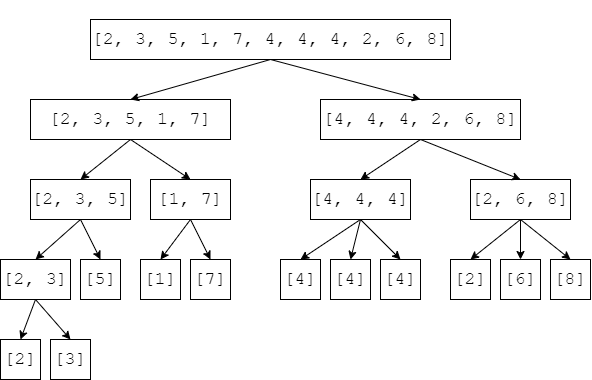
\includegraphics[width=10cm]{07-MergeSort2.drawio.png}

                    \item At the bottom nodes, you can observe arrays of size 1
                \end{itemize}
            \end{itemize}
            \item The sorting algorithm used in most Python Implementation is called \textbf{timsort.}
            \item Timsort's worst case performance is the same as merge sort's, but on average it performs considerablty better.
        \end{itemize}
        \item The relational operators compare the Unicode values of the characters of the strings from the zeroth index till the end of the string. It then returns a boolean value according to the operator used. \href{https://www.geeksforgeeks.org/string-comparison-in-python/}{String Comparison}
        \item Both list.sort and sorted function can have two additional parameters. The key parameter plays the same role as in our implementation of merge.sort: it supplies the comparison function to be used.
        \begin{verbatim}
        L = [[1,2,3],(3,2,1,0),'abc']
        print(sorted(L,key=len,reverse=True))
        # sorts the element of L in reverse order of length and prints

        # Output is
        [(3, 2, 1, 0), [1, 2, 3], 'abc']
        \end{verbatim}
        \item \textbf{Hash Tables}
        \begin{itemize}
            \item The hash value is an integer which is used to quickly compare dictionary keys while looking at a dictionary.
            \item Dictionaries use a technique called hashing to do the lookup in time that is nearly indpendent of the size of the dictionary.
            \item We convert the key to an integer, and then use that integer to index into a list, which can be done in constant time.
            \item Internal Representation of string 'abc' is
            \begin{verbatim}
            >>> list(map(bin,bytearray('abc','utf8'))) 
                ['0b1100001', '0b1100010', '0b1100011']

            >>> ''.join(list(map(bin,bytearray('abc','utf8'))))  
                '0b11000010b11000100b1100011'

        'utf8' is the encoding type
        bin is Binary conversion
        bytearray returns a bytearray object (i.e. array of bytes)
            \end{verbatim}
            \item A hash function maps a large space of inputs(e.g. all natural numbers) to a smaller space of outputs(e.g. the natural numbers between 0 and 5000).
            \item They can be used to convert a large space of keys to a smaller space of integer indices.
            \item Hash function is a \textbf{many-to-one mapping.} i.e., multiple different inputs may be mapped to the same output.
            \item When two inputs are mapped to the same output, it is called \textit{collision}.
            \item A good hash function produces a \textit{uniform distribution} i.e., every output in the range is equally probable, which minimizes the probability of collisions.
            \item The basic idea is to represent an instance of class intDict by a list of \textit{hash buckets} where each bucket is a list of key/value pairs implemented as tuples.
        \end{itemize}
    \end{enumerate}
\end{document}